\documentclass[tikz,border=7pt]{standalone}
\begin{document}
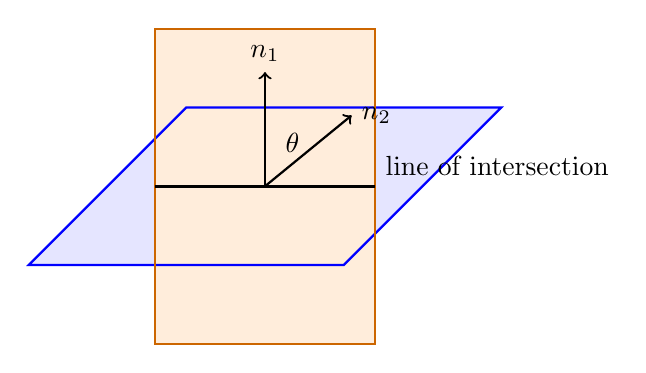
\begin{tikzpicture}[line width=.8pt]
\fill[blue!10] (-3,-1)--(1,-1)--(3,1)--(-1,1)--cycle;
\fill[orange!14] (-1.4,-2)--(1.4,-2)--(1.4,2)--(-1.4,2)--cycle;
\draw[blue] (-3,-1)--(1,-1)--(3,1)--(-1,1)--cycle;
\draw[orange!80!black] (-1.4,-2)--(1.4,-2)--(1.4,2)--(-1.4,2)--cycle;
\draw[very thick] (-1.4,0)--(1.4,0); \node[above right] at (1.4,0) {line of intersection};
\draw[->] (0,0)--(0,1.45) node[above] {$n_1$}; \draw[->] (0,0)--(1.1,.9) node[right] {$n_2$};
\node at (.35,.55) {$\theta$};
\end{tikzpicture}
\end{document}
